%% LyX 2.2.1 created this file.  For more info, see http://www.lyx.org/.
%% Do not edit unless you really know what you are doing.
\documentclass[english,sigconf]{acmart}
\usepackage[T1]{fontenc}
\usepackage[latin9]{inputenc}
\setcounter{secnumdepth}{3}
\setcounter{tocdepth}{3}
\usepackage{color}
\usepackage{amsmath}
\usepackage{graphicx}
\usepackage{multirow}
\usepackage{multicol}

\makeatletter

%%%%%%%%%%%%%%%%%%%%%%%%%%%%%% LyX specific LaTeX commands.
%% Because html converters don't know tabularnewline
\providecommand{\tabularnewline}{\\}

%%%%%%%%%%%%%%%%%%%%%%%%%%%%%% User specified LaTeX commands.


\usepackage{booktabs}% For formal tables
\usepackage{float}
\DeclareMathOperator*{\argmax}{argmax}
\DeclareMathOperator*{\argmin}{argmin}

\usepackage{rotating}
\usepackage{array}
\newcolumntype{L}[1]{>{\vspace{0.5em}\begin{minipage}{#1}\raggedright\let\newline\\
\arraybackslash\hspace{0pt}}m{#1}<{\end{minipage}\vspace{0.5em}}}
\newcolumntype{R}[1]{>{\vspace{0.5em}\begin{minipage}{#1}\raggedleft\let\newline\\
\arraybackslash\hspace{0pt}}m{#1}<{\end{minipage}\vspace{0.5em}}}
\newcolumntype{C}[1]{>{\vspace{0.5em}\begin{minipage}{#1}\centering\let\newline\\
\arraybackslash\hspace{0pt}}m{#1}<{\end{minipage}\vspace{0.5em}}}


\copyrightyear{2017}
\acmYear{2017}
\setcopyright{acmcopyright}
\acmConference{}{}{} 
\acmPrice{15.00} 
\acmDOI{http://dx.doi.org/xxx}
\acmISBN{ACM ISBN xxx}

\clubpenalty=10000 
\widowpenalty = 10000

\makeatother

\usepackage{babel}
\begin{document}
\title{A Cost-based Approach for Fast Intrusion Detection }


\author{Jiarui~Gao$^1$}

\affiliation{
\institution{$^1$School of Computer Science, Shanghai Key Laboratory of Intelligent Information Processing,\\ Fudan University, China}   
}
\email{jrgao14@fudan.edu.cn}   


\begin{abstract} 

The aim of Intrusion Detection System(IDS) is to maximize detection accuracy as well as minimize corresponding costs. In this paper, I present a cost-based approach utilizing neural network with GPU acceleration for fast intrusion detection. In this approach, both computational cost and time cost are considered, and models are trained with respect to their different protocol types and services. Empirical experiments are carried out on off-line benchmark dataset NSL-KDD.

\end{abstract}
\keywords{Neural network; Intrusion detection; anomaly detection; cost analysis.}

\maketitle

\section{Introduction}
With the development of computing and Internet technology, Internet has became an important part of our daily life. However, this popularity has also brought security issues. 
Intrusion Detection Systems(IDSs) are designed to detect attacks, which help discover, determine, and identify unauthorized use, duplication, alteration, and destruction of information systems\cite{mukkamala2005cyber}. Specifically, IDSs are able to monitor intrusions and alert network administrators if necessary.

According to the detectable attacks, there are mainly three types of IDSs: misuse-based, anomaly-based, and hybrid\cite{buczak2016survey}.
Misuse-based IDSs are designed to detect known attacks by comparing signatures of those attacks and those in the database.
Anomaly-based IDSs have the ability for detecting zero-day attacks. The normal network are modeled and anomalies can be detected when happened.

Also with respect for using environment, IDSs can be used in real-time environment of off-line environment. Off-line IDSs have been studied extensively recently. 
However, these systems fail to provide real time information, which means they can only detect intrusions after they already happened. The challenge for real-time IDSs is the huge cost brought with the detection.

In this paper, the aim is to develop a IDS which can be utilized in real-time environment with high detection accuracy. I present a cost-based approach for anomaly intrusion detection. The traditional machine learning models are replaced by neural networks, which enable the computational cost to be minimized utilizing GPU acceleration. 
Also, the time cost is considered, and according to the time cost theory in \cite{lee2001real}, low level features are utilized with high priority. The benchmark dataset NSL-KDD is used for evaluation, which is a new version of dataset KDDCUP'99\cite{cup2007available} and has significant improvements compared with KDDcup99\cite{tavallaee2009detailed}.

The rest of the paper is organized as follows. Sec \ref{sec:relatedwork} gives a detailed review of current related work about intrusion detection. In Sec \ref{sec:methodology}, the new approach for intrusion detection is introduced. The experimental results are reported in Sec \ref{sec:experiment}. More future work is presented in Sec \ref{sec:futurework}. Finally, a conclusion is drew in Sec \ref{sec:conclusion}.

\section{Related Work}\label{sec:relatedwork}
\subsection{Detection Methodology}


\subsection{Machine Learning for Intrusion Detection}


\subsection{Public Datasets}\label{sec:publicdatasets}

\section{Methodology}\label{sec:methodology}

As shown in Fig \ref{fig:overview}, a multi-model detector is presented here.

\begin{figure*}[t]
\begin{centering}
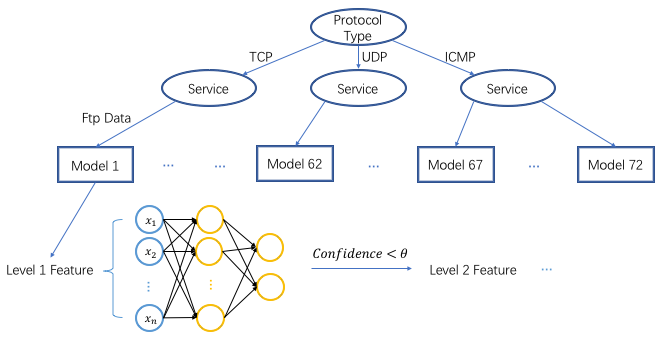
\includegraphics[scale=0.5]{img/overview}
\par\end{centering}
\caption{\label{fig:overview} An overview of the detection framework including the decision tree(top part) and the neural networks(bottom part). The total number of models are calculated on NSL-KDD dataset.}
\end{figure*}


\subsection{Cost Analysis}

\textbf{Computational Cost.}\quad One of the major challenges in real-time IDSs is the computational cost attached with the system. For example, the well-known K-nearest Neighbor Classifier\cite{liao2002use} performs well on off-line datasets, but it is not an appropriate detector in real time. Because the
KNNC calculates the similarity between the new 
process and each process in the training set to decide the label of the new process. So KNNC is computationally
expensive when the incoming number of processes is huge.

Traditionally, less features and models with less parameters will lead to low computational cost. However, this may also result in lower detection accuracy or higher false alarm rate. Different from former approaches, utilizing deep neural networks, the computing tasks can be accelerated on GPU\cite{chetlur2014cudnn}. Also, the ability to represent any non-linear function in very few hidden layers and hidden neurons make the computational expense even less.

\noindent\textbf{Time Cost.}\quad It is obvious that the time delay for retrieving features simply from a network packet and extracting information from all former similar connections within a time period are quite different. Different from\cite{lee2001real}, the connection based features are utilized according to\cite{lee2001real} in this paper.

\begin{itemize}
\item Level 1 features are basic features of individual TCP connections.
\item Level 2 features are content features within a connection suggested by domain knowledge.
\item Level 3 features are traffic features computed using a two-second time window.
\end{itemize}

Notice that the Level 3 features require iteration from the entire former two-second packet set, the time cost is extremely high. Also, all the Level 3 features for connections coming at the same time can also be computed at the same time.

The lower level features are first used, and if the confidence of the classification is less than a threshold $\theta$, higher level features are extracted and are used combined with other lower level features. For example, both Level 1 and Level 2 features are considered after extracting the Level 2 features.

\subsection{Neural Network Detectors}

Packets with different protocol types and different services tend to have different signatures to be malicious. So neural network models are trained for each protocol type and service respectively.
Thus for each new connection, its protocol type and service decides which detector to use. This model selection framework can be modeled by a decision tree. 

Neural network models with only one hidden layer is utilized in this paper, and the following experiments proves their capability for intrusion detection with such simple architectures.

\section{Experiments}\label{sec:experiment}
\subsection{Dataset}
As mentioned in Sec \ref{sec:publicdatasets}, NSL-KDD dataset consists of the selected records of the KDDCUP'99 dataset, which is more challenging to detect compared with the original widely used benchmark KDDCUP'99 dataset. 
The NLS-KDD dataset solves the issues of models trained on KDDCUP'99 dataset, which have high seemingly accuracy but actually poor capability of anomaly detection.

All the features in NSL-KDD dataset are considered in this paper except the additional feature: detection difficulty, which is generalized by statistical analysis for the KDDCUP'99 dataset\cite{tavallaee2009detailed}. Totally, there are $61$ different TCP services, $5$ different UDP services and $6$ different ICMP services.

\subsection{Parameter setting}
All the code is implemented in Python utilizing deep learning framework Tensorflow, and the neural network models are trained on one GPU GeForce GTX TITAN X for $5000$ epochs with early stop policy. All the neural networks consist of $1$ hidden layer, and the number of hidden neurons are set specifically for every model. The initial learning rate is $\eta = 0.0001$ and dropout ratio is $0.75$. Finally, a softmax layer with two output values is utilized to calculate loss and Adam\cite{kingma2014adam} is used to accelerate learning.

\subsection{Baseline}
Support Vector Machine(SVM) is utilized as a baseline method for each model respectively. The code are implemented in Python on Scikit-learn Library. And the following baseline results are evaluated on the same server with the proposed approach without GPU support for SVM method.

\subsection{Detection Results}
Due to the coming deadline issue, I have only finished part of the experiments.

\textbf{Detection Accuracy.}
Tab \ref{tab:detection-accuracy} demonstrates the detection accuracy for each level of features. And apart from the over all accuracy, I take three representative protocol type and service(TCP finger/UDP domain\_u/ICMP eco\_i) as examples.

Observed from Tab \ref{tab:detection-accuracy}, we can see that SVM models and neural network models perform nearly the same on most of the detections. But neural network models demonstrate a good property that as the level of features get higher, the accuracies never decay; while the SVM method present less stability. 

Also, we can observe that the decision tree idea that to detect different protocol types and service with different models is quite reasonable. In Tab \ref{tab:detection-accuracy}, huge accuracy improvement has been made thanks to this separation.

\begin{table*}

\caption{\label{tab:detection-accuracy}Detection Accuracy Results.}
\centering{}
\begin{tabular}{ccccc}

\hline 
Methods/Features & Over all & TCP finger & UDP domain\_u & ICMP eco\_i \tabularnewline
\hline
\textbf{Level 1 Features} \tabularnewline
SVM & $78.20\%$ & $99.26\%$ & $99.33\%$ & $94.27\%$ \tabularnewline
Ours & $77.26\%$ & $99.26\%$ & $99.33\%$ & $94.27\%$\tabularnewline
\hline

\textbf{Level 2 Features} \tabularnewline
 
SVM & $81.39\%$ & $97.06\%$ & $99.55\%$ & $94.27\%$\tabularnewline
Ours & $80.67\%$ & $99.26\%$ & $99.78\%$ & $94.27\%$\tabularnewline
\hline

\textbf{Level 3 Features} \tabularnewline
  
SVM & $80.57\%$ & $99.26\%$ & $99.78\%$ & $98.09\%$\tabularnewline
Ours & $76.24\%$ & $99.26\%$ & $99.78\%$ & $98.89\%$\tabularnewline
\hline
\end{tabular}
\end{table*}

\textbf{Cost Analysis.}
Tab \ref{tab:cost} demonstrates the \textbf{computational cost} for each level of features. The same as former experiments, three representative protocol type and service are selected. Notice here I report the average time for computing single one packet feature item. 

It can be noticed that significant improvement have been on computational cost utilizing neural network models, which is quite important in real time detection ability for the IDSs.

Also, the \textbf{time cost} is considered. Each new packet are first detected according to their Level 1 features. If the confidence of the classification, which is the larger value of the two output neurons is less than $\theta=0.8$, than the higher features are extracted and higher level models are used. 
In the worst case, the packet will eventually get its label through Level 3 models. And more additional computational cost will also be spent. 

The total cost is the sum of computational cost and time cost, which is much more efficient compared with simply using Level 3 features for all the packets.

\begin{table*}

\caption{\label{tab:cost}Computational Cost Results.}
\centering{}
\begin{tabular}{ccccc}

\hline 
Methods/Features & Over all & TCP finger & UDP domain\_u & ICMP eco\_i \tabularnewline
\hline
\textbf{Level 1 Features} \tabularnewline
SVM & $4.2*10^{-4}s$ & $4.4*10^{-6}s$ & $9.2*10^{-7}s$ & $5.7*10^{-7}s$ \tabularnewline
Ours & $5.4*10^{-8}s$ & $2.7*10^{-6}s$ & $4.3*10^{-7}s$ & $1.4*10^{-6}s$\tabularnewline
\hline

\textbf{Level 2 Features} \tabularnewline
 
SVM & $5.9*10^{-4}s$ & $7.3*10^{-6}s$ & $1.3*10^{-6}s$ & $1.3*10^{-6}s$\tabularnewline
Ours & $7.0*10^{-8}s$ & $2.7*10^{-6}s$ & $4.6*10^{-7}s$ & $1.4*10^{-6}s$\tabularnewline
\hline

\textbf{Level 3 Features} \tabularnewline
  
SVM & $2.3*10^{-4}s$ & $7.2*10^{-6}s$ & $4.1*10^{-6}s$ & $6.2*10^{-6}s$\tabularnewline
Ours & $1.0*10^{-7}s$ & $2.8*10^{-6}s$ & $5.2*10^{-7}s$ & $1.5*10^{-6}s$\tabularnewline
\hline
\end{tabular}
\end{table*}


\section{Future Work}\label{sec:futurework}
As mentioned in Sec \ref{sec:experiment}, due to the coming deadline, some of the experiments are not completely finished. 

The future work for this paper is listed as follows:
\begin{itemize}
\item Calculate the average performance for all the models, not for only some examples.
\item Measure the specific improvement made by distinguishing different level of features quantitatively, such as calculate the exact cost saved for detecting some packets.
\end{itemize}

There are also some practical need to be solved for further implementation:
\begin{itemize}
\item There are some protocol type and service with very few training data, such as TCP pm\_dump, UDP tftp\_u and ICMP urh\_i etc. This issue will make it impossible to train a neural network model. Maybe some signature-based technique are needed here.
\item It will cost too much time to train and tune parameters for every model, specifically $72$ models in NSL-KDD dataset. But currently I just train the example models manually.
\end{itemize}

\section{Conclusion}\label{sec:conclusion}


\bibliographystyle{ACM-Reference-Format}
\bibliography{security} 
\end{document}